\chapter{Mitigate Fingerprinting of Honeypots}
\label{chap:fingerprinting}

... % TODO: Add introduction, explain ssh \section{Introduction}

Our experiment exists out of two steps.
First, we want to reproduce the cosine similarity coefficient that \citet{vetterl2020} claims.
Second, we want to disguise Cowrie with the idea we have mentioned beforehand.

\section{OpenSSH}
\label{sec:openssh}

OpenSSH is one of the widely used applications to acquire an SSH connection.
Before proceeding with generic weaknesses of SSH honeypots, we want to give a short intermezzo about OpenSSH itself.

\begin{figure}[ht]
    \centering
    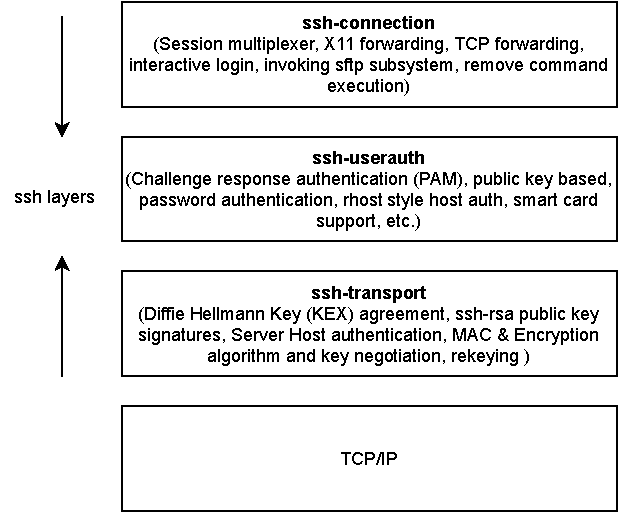
\includegraphics{figures/openssh-architecture.pdf}
    \caption[OpenSSH architecture]{OpenSSH architecture (derived from \cite{openssh2007})}
    \label{fig:openssh-architecture}
\end{figure}

OpenSSH consists of three major layers, namely \verb|ssh-connection|, \verb|ssh-userauth|, and \verb|ssh-transport|.
Last layer is the most important one because it provides the basic functionalities for crypto operations such as the key exchange.

The first layer is responsible for authenticating the user to the sshd daemon.
Due to two-way authentication, the client authenticates the sshd daemon by the help of the \verb|ssh-transport|.
Finally, a secure connection is established, and the key exchange is done.
Next step is to authenticate the user.
Therefore, it offers various authentication methods such as username/password authentication.
If the \verb|ssh-userauth| layer is successful, it will establish a secure channel through the \verb|ssh-connection| layer.
Each connection is handled in a channel that is used for the user's session.

The \verb|ssh-connection| layer handles multiple sessions simultaneously over a single \verb|ssh-userauth| layer with the TCP/IP layer below.
It is responsible for executing arbitrary commands, forwarding X11 connections, establishing VPN tunnels and more.

In addition, OpenSSH comes with built-in features such as keep alive messages, redirecting stdin to /dev/null for specialized X windows.

\begin{figure}[ht]
    \centering
    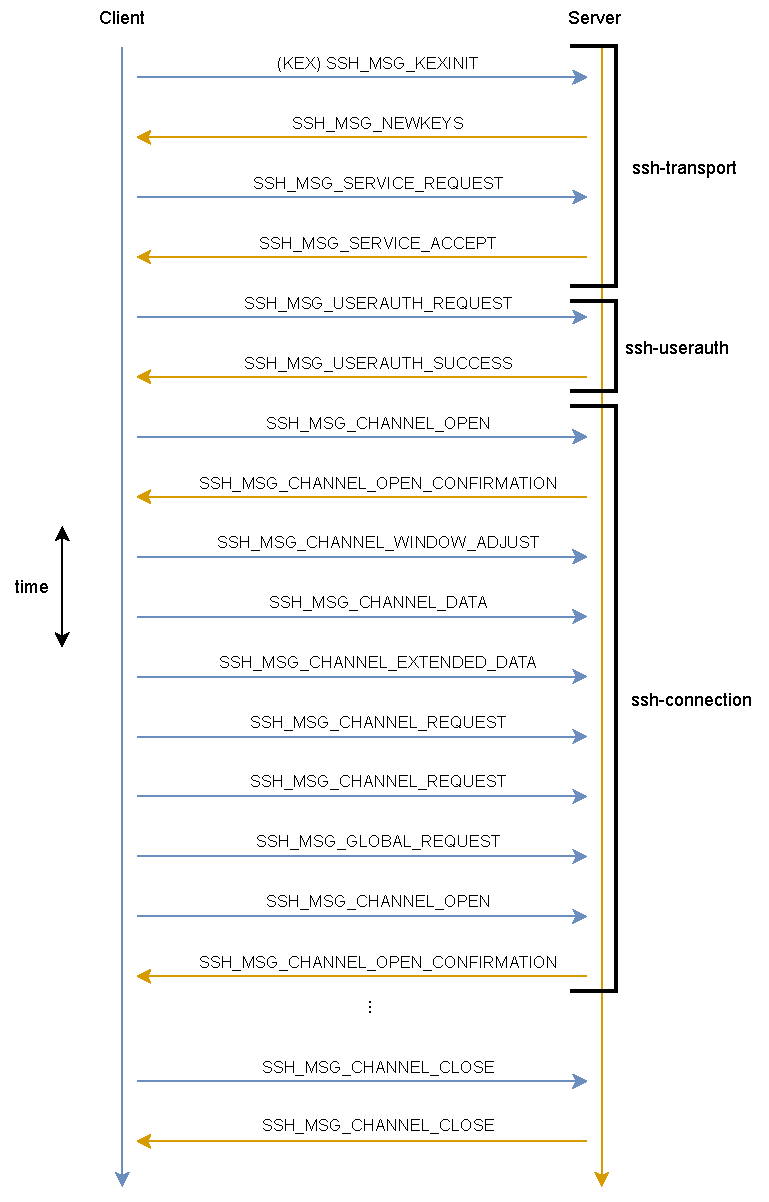
\includegraphics{figures/ssh-flow-diagram.pdf}
    \caption[OpenSSH sample session flow diagram]{OpenSSH sample session flow diagram (derived from \cite{openssh2007}). In addition, on the right side indicates the layers that are responsible for handling the messages.}
    \label{fig:openssh-flow-diagram}
\end{figure}

\autoref{fig:openssh-flow-diagram} shows a sample session.

\section{Preliminary Work}

Attackers have a strong motivation to reveal honeypots before launching an attack.
Without any protection attackers would disclose their methods, and thus, newly developed attacks would become useless.
As shown in \autoref{chap:cloud-security}, attackers do try to get information about the host system.
\citet{vetterl2020} discussed various methods of fingerprinting, however, executing commands in a login shell and examining the response leaves precarious information to the honeypot itself.
In his work he evaluated methods to detect honeypots at the transport level.
As stated, the value of a honeypot would be merely zero if a detection on transport level would work.
He presents fingerprinting methods for SSH, Telnet, and HTTP/Web.
Due to the complexity of each method, we focus on SSH fingerprinting with the honeypot Cowrie.
The idea to detect SSH honeypots is to look for deviations in the response.
Therefore, \citet{vetterl2020} sends a set of probes $P = \{P_1, P_2, \dots, P_n\}$ to a given set of implementations of a network protocol $I = \{I_1, I_2, \dots, I_n\}$ and stores the set of responses $R = \{R_1, R_2, \dots, R_n\}$.
For the given set of responses he calculated the cosine similarity coefficient $C$.
Goal is to find the best $P_i$ where the sum of $C$ is the lowest.
\autoref{fig:draft-cosine-similarity} presents these steps.

Cosine similarity outputs the similarity between vectors of numerical attributes.
In text semantics it is widely used to measure the similarity of sets of information such as two sentences.
\citet{vetterl2020} outlines that it can be used in \enquote{traffic analysis to find abnormalities and to measure domain similarity}.
Mathematically, it computes the angle between two vectors.
For each set of information $A$, we create a vector $D_A$.
Referring to our use case with SSH, we use the response from the server as information $A$.
If $\theta$ is the angle between $D_A$ and $D_B$, then:

\begin{equation} \label{eq:cosine-similarity}
    \cos \theta = \frac{D_A \cdot D_B}{\|D_A\| \|D_B\|}
\end{equation}

where \enquote{$\cdot$} is the dot product obtained by:

\begin{equation}
    D_A \cdot D_B = \sum_{i=1}^{n} (D_{A_i} \times D_{B_i})
\end{equation}

and $\|D_A\|$ (resp. $\|D_B\|$) is the Euclidean norm, obtained by $\sqrt{\sum_{i=1}^{n} D_{A_i}^2}$ (resp. $\sqrt{\sum_{i=1}^{n} D_{B_i}^2}$).
The values of vectors are non-negative. The similarity between items is the value $\cos \theta$, $\cos \theta = 1$ indicates equality.

\begin{figure}[ht]
    \centering
    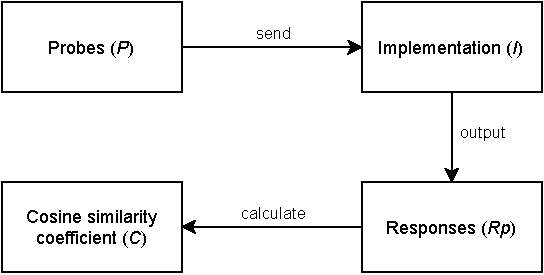
\includegraphics{figures/vetterl_concept.pdf}
    \caption[Outline to obtain the cosine similarity coefficient]{Outline to obtain the cosine similarity coefficient (derived from \cite{vetterl2020}).}
    \label{fig:draft-cosine-similarity}
\end{figure}

In order to find the best $P_i$ for SSH, \citet{vetterl2020} first created different SSH version strings based on the format: \verb|SSH-protoversion-swversion SP comment crlf|.
He used different lower and upper case variations, 12 different protoversions ranging from $0.0$ to $3.2$, swversion set to \enquote{OpenSSH} or empty string, comment set to \enquote{FreeBSD} or empty string, and crlf to either \verb|\r\n| or empty string.
In total, summing up to 192 client version strings.
Second, he created different \verb|SSH2_MSG_KEXINIT| packets with 16 key-exchange algorithms, 2 host key algorithms, 15 encryption algorithms, 5 MAC algorithms and 3 compression algorithms.
In total, he sent \numprint{58752} \verb|SSH2_MSG_KEXINIT| packets.
Combining them with the 192 client versions, he ended up sending \numprint{157925376} packets.
The version string \verb|SSH-2.2-OpenSSH \r\n| and the \verb|SSH2_MSG_KEXINIT| packet including ecdh-sha2-nistp521 as key-exchange algorithm, ssh-dss as host key algorithm, blowfish-cbc as encryption algorithm, hmac-sha1 as mac algorithm and zlib@openssh.com as compression algorithm, with the wrong padding result in the lowest cosine similarity coefficient $C$.
\autoref{lst:ssh-debug} shows the SSH debug information with the modified version string, and key exchange message.

\begin{figure}
    \lstinputlisting[language=bash, caption={OpenSSH connection attempt with probed SSH packet. All non-essential debug information have been removed to lay emphasis on the modified key exchange initialization.}, label={lst:ssh-debug}]{listings/ssh-debug.txt}
\end{figure}

\autoref{tab:cosine-similarity} has been derived from \citet{vetterl2020} to present his results of the cosine similarity of OpenSSH, Twisted, and Cowrie.
Twisted has been added to have an example with an older SSH honeypot.
We can see that it differs fundamentally from OpenSSH.
At most, it scores $0.52$ whereas various OpenSSH versions start at $0.98$.
The number of hosts significantly decrease with a cosine similarity score of $0.90$ and higher.
Cowrie responses are not too far away to OpenSSH with an average of $0.80$.
However, scanning through the web with a minimum score of $0.90$ and higher would exclude all honeypots.
Thus, distinguishing Cowrie from OpenSSH with SSH packets is a feasible method.
Moreover, \citet{vetterl2020} performed an Internet-wide scan, and detected $758$ Kippo and $2021$ Cowrie honeypots.
These results show that the values of honeypots would decrease to zero when large fingerprinting activities are used.

\begin{figure}[ht]
    \centering
    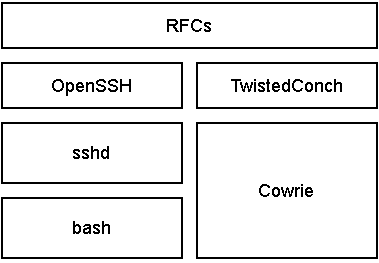
\includegraphics{figures/cowrie-openssh.pdf}
    \caption[Architecture of OpenSSH and Cowrie]{Architecture of OpenSSH and Cowrie. OpenSSH and TwistedConch have subtle differences (derived from \cite{vetterl2020})}
    \label{fig:cowrie-openssh}
\end{figure}

\citet{vetterl2020} states that current low- and medium-interaction honeypots have a generic weakness due to the underlying off-the-shelf libraries.
Cowrie is based on TwistedConch, a Python 2/3 library that implements the SSH protocol.
Any bash command and its response are tweaked by Cowrie, and thus, resulting in a discrepancy to OpenSSH.
For example, Cowrie version $1.1.0$ missed \verb|tftp|\footnote{Is } and came with version $1.2.0$.
Therefore, it is a continuous struggle of adding new commands to avoid early disclosures of Cowrie.

\autoref{fig:cowrie-openssh} shows the difference between OpenSSH and Cowrie.
Both have to fulfill the RFC 4250 \cite{rfc4250} requirement on top.
OpenSSH and TwistedConch implement the SSH protocol.
As an example, \citet{vetterl2020} found that Cowrie used to have random bytes for the \verb|SSH2_MSG_KEXINIT| packet\footnote{Each packet consists of the packet and padding length, the \ac{mac}, a payload, and a random padding.} unlike OpenSSH.
With respect to RFC4253 \cite{rfc4253} that defines the \ac{bpp} of SSH, the random padding is used to solidify the total length of the packet to be a multiple of the cipher block size.
The RFC in section 6 defines that the padding have to consist of 4 random bytes.
Based on the statement of the OpenSSH authors, random bytes have been changed to \verb|NULL| characters due to no security implications.
Thus, an adversary could have detected a Cowrie honeypot with a single \verb|SSH2_MSG_KEXINIT| packet.
Nowadays, Cowrie adapted itself to have \verb|NULL| characters as padding.
However, these subtle differences influence the cosine similarity coefficient.

\begin{table}
    \caption{Overview of the cosine similarity of OpenSSH, Cowrie, and Twisted}
    \begin{tabular}{lc|cccccccccc}
    \toprule
                   &   & A & B      & C      & D      & E      & F      & G      & H      & I      & J      \\
    \hline
    OpenSSH 6.6    & A & - & $0.98$ & $0.98$ & $0.94$ & $0.94$ & $0.42$ & $0.78$ & $0.79$ & $0.79$ & $0.79$ \\
    OpenSSH 6.7    & B &   & -      & $0.98$ & $0.98$ & $0.98$ & $0.41$ & $0.80$ & $0.81$ & $0.81$ & $0.80$ \\
    OpenSSH 6.8    & C &   &        & -      & $0.96$ & $0.96$ & $0.42$ & $0.78$ & $0.79$ & $0.79$ & $0.79$ \\
    OpenSSH 7.2    & D &   &        &        & -      & $0.98$ & $0.42$ & $0.80$ & $0.80$ & $0.80$ & $0.80$ \\
    OpenSSH 7.5    & E &   &        &        &        & -      & $0.42$ & $0.78$ & $0.79$ & $0.79$ & $0.79$ \\
    \\
    \cline{1-2} \cline{8-12}
    \\
    Twisted 15.2.1 & F &   &        &        &        &        & -      & $0.50$ & $0.51$ & $0.51$ & $0.52$ \\
    \\
    \cline{1-2} \cline{9-12}
    \\
    Cowrie 96ca2ba & G &   &        &        &        &        &        & -      & $0.98$ & $0.98$ & $0.98$ \\
    Cowrie dc45961 & H &   &        &        &        &        &        &        & -      & $0.99$ & $0.99$ \\
    Cowrie dbe88ed & I &   &        &        &        &        &        &        &        & -      & $0.99$ \\
    Cowrie fd801d1 & J &   &        &        &        &        &        &        &        &        & -      \\
    \bottomrule
    \end{tabular}
    \label{tab:cosine-similarity}
\end{table}

\section{Experiment 1: Reproduce Vetterl et al.'s findings}

First, the reproduction of the outdated OpenSSH library that \citet{vetterl2020} used will be investigated.
In his work he used OpenSSH $7.5P1$ which deviates from the latest version $8.8P1$.
Older versions rely on OpenSSL $1.0.2$ which includes outdated algorithms and functions.
For the \verb|SSH2_MSG_KEXINIT| packet, the encryption algorithm blowfish-cbc has been removed with version $7.6P1$, and thus, are outdated.
Building the version $7.5P1$ requires the libraries libssl (1.0.2), libssl-dev (1.0), libssh-dev (0.7.3-2), and libssh-4 (0.9.6-1).
Using the latest versions of these libraries result in errors such as missing encryption algorithms and host key algorithm.
After compiling the package, we test its behavior with a Debian 11 Buster and a Debian Jessie 9 Docker image.
Both are new machines that have no other packages installed than the OpenSSH server.
Debian 11 uses the latest OpenSSH version whereas Jessie is at $6.7P1$.
These environments help us to uniquely identify variations in the protocol version.

\begin{figure}
    \lstinputlisting[language=bash, caption={OpenSSH connection attempt with probed SSH packet}, label={lst:ssh-openssh}]{listings/ssh-openssh.txt}
\end{figure}

\autoref{lst:ssh-openssh} shows the connection attempt with our adjusted version string and \verb|SSH2_MSG_KEXINIT| packet.
Both Debian machines have the same response.
Using the outdated OpenSSH version $7.5P1$ results in an incompatibility.
OpenSSH outlines that blowfish-cbc is not supported anymore.
OpenSSH kept the encryption algorithm usable for compatibility reasons for clients until $7.6P1$.
Later, patches removed the blowfish-cbc from the SSH server, and thus, a reproduction of \citet{vetterl2020} remains not feasible with state-of-the-art OpenSSH versions.
However, testing it with version $7.3P1$ that has been compiled on the machine results in a successful connection attempt.
\citet{vetterl2020} does not outline any expected response of OpenSSH, thus, we can just assume that a connection attempt would have been successful due to the existing ciphers during that time.
Adapting OpenSSH version $8.8P1$ with chacha20-poly1305 instead of blowfish-cbc and results in a successful connection attempt.
For instance, we have adapted the key exchange initialization to use chacha20-poly1305 as encryption algorithm instead.
Next, the DSA host key algorithms are marked as too weak, and are not include automatically.
Using ssh-dss requires the extra flag \verb|-oHostKeyAlgorithms=+ssh-dss|.
In addition, we have tested it with the ssh-rsa host key algorithm, and the response has been promising to probe instances.
This adaption with the \verb|SSH2_MSG_KEXINIT| packet including ecdh-sha2-nistp521 as key-exchange algorithm, ssh-dss as host key algorithm, chacha20-poly1305 as encryption algorithm, hmac-sha1 as mac algorithm and zlib@openssh.com as compression algorithm has been successfully tested on our two Debian instances.
Respectively, for OpenSSH version $8.8P1$ we have updated the fingerprinting method by replacing the encryption algorithm.

\begin{figure}
    \lstinputlisting[language=bash, caption={Cowrie connection attempt with probed SSH packet}, label={lst:ssh-cowrie}]{listings/ssh-cowrie.txt}
\end{figure}

Most interesting question remains the response deviation of Cowrie.
For instance, we use the default Cowrie implementation version $v.2.3.0$\footnote{\url{https://github.com/cowrie/cowrie/commit/555ff10d95f6239d9d6efee8a2d05def316ab144}} of our T-Pot instance.
\autoref{lst:ssh-cowrie} outlines the connection attempt of Cowrie.
Unambiguously, Cowrie results in a  \verb|bad packet length *| exception, and thus, deviates fundamentally from an OpenSSH response.
The underlying off-the-shelf library TwistedConch checks if a packet is within $1048576$ bytes (1 MB).
Any packet that exceeds that limit causes a \verb|bad packet length *| exception that results in a connection loss of the client.
When Cowrie tries to get the packet of a request this static check (\autoref{lst:twistedconch}) will be performed.
It remains dubious why TwistedConch has added it whenever an SSH packet has to be returned.
In the RFC 4253, the minimum packet size is $5$ bytes whereas maximum packet size is set to $32768$ bytes (256 KB).
Debugging Cowrie shows that the exception occurs during the version string validation.
The server validates if the version string matches the allowed versions $1.99$ and $2.0$.
Any version higher or lower than the allowed versions result in a \verb|Protocol major versions differ.\n| exception.
This response matches the behavior of OpenSSH.
\citet{vetterl2020} claims that TwistedConch results in a \verb|bad version *| exception, however, in the meantime this issue has been fixed by Cowrie, and thus, do not leak vulnerable information anymore.
For instance, we have tested Cowrie and OpenSSH with the version $1.0$, $2.0$ and $2.2$. 
As a result, for Cowrie the \verb|bad packet length *| exception only occurs when the version does not match the expected ones.
This result diverges from OpenSSH.
For OpenSSH only versions lower than $1.99$ results in the same exception as Cowrie.
For any higher version, the connection can be acquired successfully.
We assume that Cowrie has a bug during the version string validation.
These are the protocol deviations that \citet{vetterl2020} has presented in his work.
Thus, detecting honeypots on transport level has been confirmed.
Adversaries who modify their SSH client to send our specific version string and key exchange initialization message could detect Cowrie honeypots and stop any further activity.

\begin{figure}
    \lstinputlisting[language=python, caption={TwistedConch packet length validation}, label={lst:twistedconch}]{listings/twistedconch.txt}
\end{figure}

\begin{figure}
    \lstinputlisting[language=python, caption={Cowrie version string validation}, label={lst:cowrie-version-string}]{listings/twistedconch.txt}
\end{figure}

\section{Attempt to Disguise Cowrie}

Cowrie has to be tweaked to hide its generic weakness.
Fixing the major flaws in Cowrie to avoid early detection remains an ephemeral patch.
Therefore, a new solution is required to disguise SSH honeypots.
Continue using libraries that re-implement the behavior of OpenSSH results in adversaries that blacklist any related host machine returning a similar cosine similarity coefficient.
\citet{vetterl2020} presented a solution to use OpenSSH as an intermediary instance between the attacker and Cowrie.
Unfortunately, this solution is outdated, and newer versions have major changes.
Thus, our concept is based on \citet{vetterl2020} honeypot, however, due to newer available versions we have updated it to the latest OpenSSH version.
OpenSSH itself is not capable by default to function as an intermediary, therefore, we have to adjust the latest OpenSSH version to enable this feature.
\autoref{fig:cowrie-fix} visualizes the flow of SSH packets between an attacker and Cowrie.
Cowrie is hidden in the background, and is only accessible through the loop back address \ipAddress{127.0.0.1:640522}.
Our updated SSH version \verb|sshd| is exposed to the Internet, and is accessible through \ipAddress{129.206.5.157:2222}.
Any connection obtain to OpenSSH will be forwarded to our honeypot.
Respectively, an attacker should not be able to detect Cowrie by response deviations because any response packet runs through OpenSSH.

% TODO: caption ueberpruefen, update mit IP etc.
\begin{figure}[ht]
    \centering
    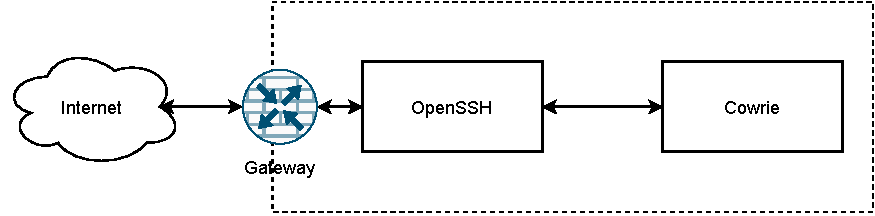
\includegraphics{figures/sshd-honeypot.pdf}
    \caption[Architecture of OpenSSH and Cowrie]{Architecture of OpenSSH and Cowrie. OpenSSH and TwistedConch have subtle differences (derived from \cite{vetterl2020})}
    \label{fig:cowrie-fix}
\end{figure}

% TODO: Code review aufzeigen
For instance, we use the latest OpenSSH version $8.8P1$.
The easiest step is to tweak the authentication to permit any connection so that an incoming connection can be forwarded to Cowrie.
Therefore, our server just returns true in the \verb|allowed_user| function to skip the rest of the authentication process.
The rest will be handled by Cowrie instead.
In OpenSSH, communications are handled in so-called channels as seen beforehand in \autoref{sec:openssh}.
Thus, a channel adaption is required for our concept.
In addition, after a successful connection the client 

\section{Experiment 2: Avoid fingerprinting of Cowrie}

\begin{figure}
    \lstinputlisting[language=bash, caption={Disguised Cowrie connection attempt with probed SSH packet}, label={lst:ssh-cowrie-fixed}]{listings/ssh-cowrie-fixed.txt}
\end{figure}

The next step is to disguise Cowrie behind an OpenSSH server.
As we have seen beforehand, the OpenSSH server should work as an intermediary between Cowrie and the attacker.
We have implemented this concept in heiCLOUD.

% TODO: Add discussion
\section{Discussion}
